\documentclass{standalone}
\usepackage{tikz}
\begin{document}
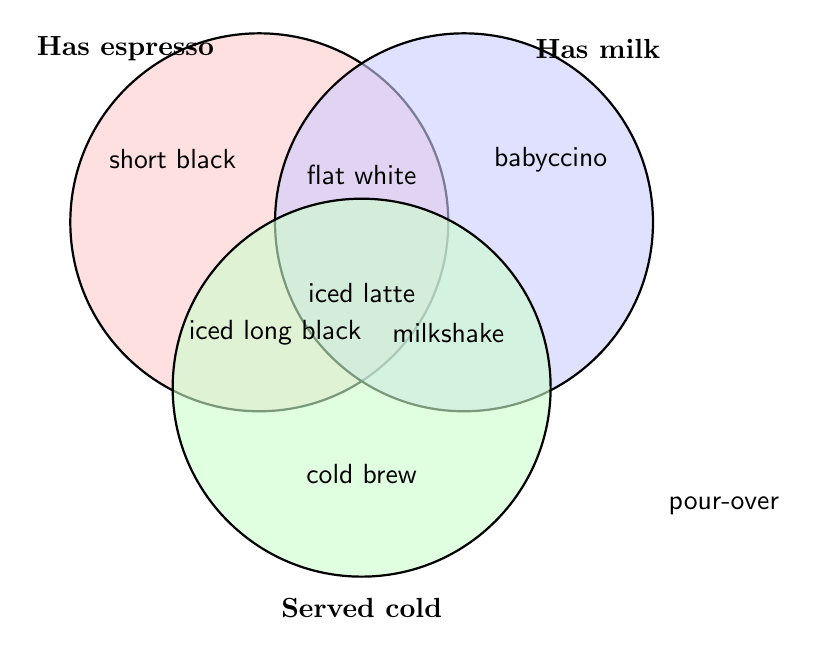
\begin{tikzpicture}[font=\sffamily]
  % Circles
  \draw[thick,fill=red!20,fill opacity=0.6]    (-1.3,0.8)  circle (2.4);
  \draw[thick,fill=blue!20,fill opacity=0.6]   (1.3,0.8)   circle (2.4);
  \draw[thick,fill=green!20,fill opacity=0.6]  (0,-1.3)    circle (2.4);

  % Labels
  \node[font=\bfseries] at (-3.0,3.0) {Has espresso};
  \node[font=\bfseries] at (3.0,3.0)  {Has milk};
  \node[font=\bfseries] at (0,-4.1)   {Served cold};

  % Drinks
  \node at (-2.4,1.6)  {short black};      % espresso only
  \node at (2.4,1.6)   {babyccino};        % milk only
  \node at (0,1.4)     {flat white};       % espresso + milk
  \node at (-1.1,-0.6) {iced long black};  % espresso + cold
  \node at (1.1,-0.6)  {milkshake};        % milk + cold
  \node at (0,-0.1)    {iced latte};       % all three
  \node at (0,-2.4)    {cold brew};        % cold only
  \node at (4.6,-2.8)  {pour-over};        % outside all
\end{tikzpicture}
\end{document}
